\section{Methods}

\subsection*{Bayesian Model}

To achieve our three objectives of 1) developing a new Bayesian pharmacokinetic model for apixaban, 2) investigating the impact of MAP versus HMC inference on dosing decisions and 3) developing an induction dosing model for apixaban, we fit a hierarchical mixed effects model of apixaban pharmacokinetics using data from \cite{Beaton2018-el}.  Thirty-six participants were given 5 mg of apixaban and 100 ml of water in a fasted state. Blood plasma concentrations of apixaban were recorded over the course of 12 hours.



\begin{table}[htb]
	\centering
	\caption{Summary of data from  \cite{Beaton2018-el}. } 
	\label{tab:my table} 
	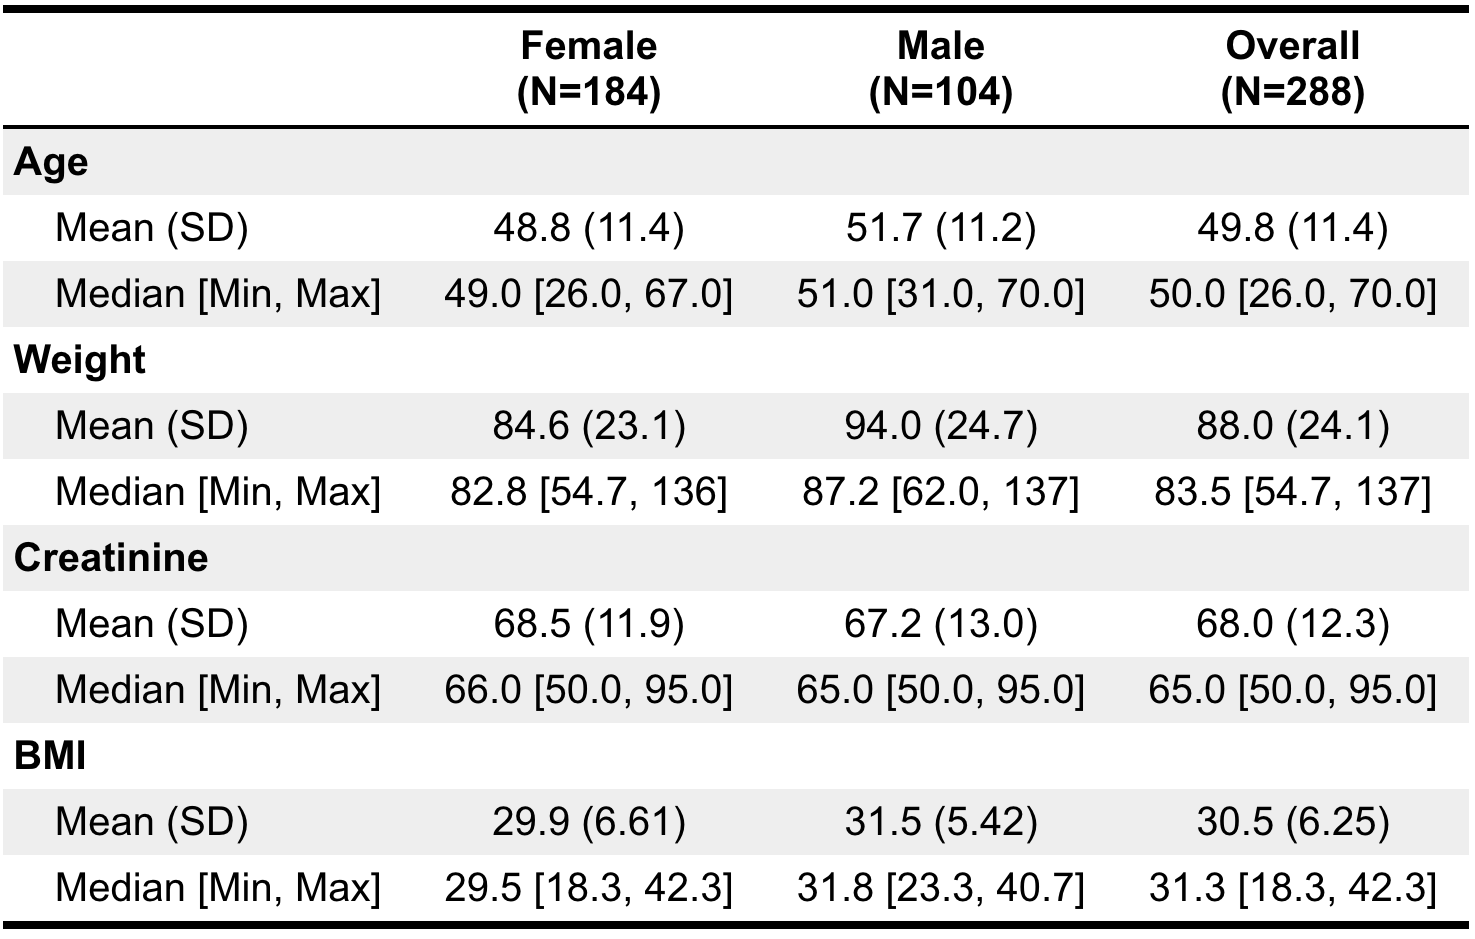
\includegraphics[width=0.7\linewidth]{figs/table1}
\end{table}


\noindent Since participants were given a single dose of apixaban in a fasted state, we use a single-compartment pharmacokinetic model with first order absorption and elimination.  The solution to the differential equation describing mass transit, and consequently the concentration function, is then


\begin{equation} \label{eq:eq_1}
y(t) =  \begin{cases}  \dfrac{F \cdot D}{Cl} \dfrac{k_e \cdot k_a}{k_e - k_a}\Bigg( e^{-k_a (t-\delta)} - e^{-k_e(t-\delta)} \Bigg)  & \delta \leq t\\\\ 0 & \mbox{else} \end{cases}
\end{equation}

\noindent Here, $D$ is the size of the dose in mg, $F$ is the bioavailability (fixed to 0.5 for apixaban \cite{Byon2019-gf}), $Cl$ is the clearance rate in units litres per hour, $k_a$ is the rate constant of absorption into the volume of distribution in units 1/hours, and $k_e$ is the elimination rate constant in units 1/hours. We include a time delay, $\delta$, to relax the assumption that absorption begins immediately after ingestion.  Parameters are considered as random effects, with some population mean and variance (which is estimated from the data). 

Priors for $k_e$ and $k_a$ are not defined explicitly.  Rather, our model puts priors on the time to max concentration, which can be expressed as a function of the parameters in \cref{eq:eq_1}

\begin{equation}\label{eq:eq_2}
 t_{max} = \dfrac{\ln(k_a) - \ln(k_e)}{k_a - k_e}
\end{equation}

\noindent and on the ratio between $k_e$ and $k_a$, which we call $\alpha$

\begin{equation}\label{eq:eq_3}
\alpha  = \dfrac{k_e}{k_a} \>.
\end{equation}

\noindent We choose to place a prior on the quantity $\alpha$ because it arises when non-dimensionalizing \citep{Lin1988-pr} the differential equation governing mass transit of the drug in and out of the volume of distribution.  The plasma concentration function is a version of the “flip-flop” model \citep{Wakefield1996-yy, Salway2008-gi}, since different parameterizations of this model can yield the same curve, leading to model un-identifiability. To ensure the model is identifiable, we require $k_e<k_a$ as has been done in previous Bayesian analyses of this model \citep{Wakefield1996-yy, Salway2008-gi}. This requirement bounds $\alpha$ to the unit interval.  In principle, information on the elimination rate constant could be obtained by performing a linear regression on the log concentration values in the latter half of the concentration profiles where the drug is being eliminated from the body. To preserve as much data as possible for model fitting, we forgo this approach.  These two sets of equations are used to parameterize the absorption and elimination rate constants as follows
\begin{align}
	k_a &= \dfrac{1}{t_{max}} \dfrac{\ln(\alpha)}{\alpha-1} \label{eq:eq_4} \\
	k_e &= k_a \alpha \label{eq:eq_5}
\end{align}

Time to max concentration values for patient $j$ are drawn from a log normal distribution

\begin{equation}\label{eq:eq_6}
t_{max, j} \vert \mu_t, \sigma_t \sim \operatorname{LogNormal}(\mu_t, \sigma_t)
\end{equation}

\noindent and $\alpha$ is drawn from a weakly informative beta prior to prevent degenerate cases when $\alpha$  is 0 or 1

\begin{equation}\label{eq:eq_7}
\alpha_j \sim \operatorname{Beta}(2,2)  \>.
\end{equation}

\noindent The rate constants for patient $j$,  $k_{e,j}$ and $k_{a,j}$, are determined from \cref{eq:eq_4,eq:eq_5}. The clearance rate is modelled hierarchically

\begin{equation}\label{eq:eq_8}
Cl_j \vert \mu_{Cl}, \sigma_{Cl}  \sim \operatorname{LogNormal}(\mu_{Cl}, \sigma_{Cl}) \>.
\end{equation}

\noindent Each patient is observed to have a non-zero concentration at time 0.5, so the time delay for each patient is no larger than 0.5 hours.  We place a beta prior on the delay

\begin{equation}\label{eq:eq_9}
\delta_j \vert \phi, \kappa \sim \operatorname{Beta}(\phi / \kappa, (1-\phi) / \kappa)
\end{equation}

\noindent and multiply delta by 0.5 in our model to ensure the maximum delay is 0.5 hours.  Here, $\phi$ is the mean of this beta distribution and $\kappa$ determines the precision of the distribution. Shown below is a Bayes net to exposit model structure at a high level.

\begin{figure}[h!]
	\centering
	\begin{tikzpicture}
	
	\node[latent](phi){$\phi$};
	\node[latent, right=of phi](kappa){$\kappa$};
	\node[latent, right = of kappa](s_t){$\sigma_t$};
	\node[latent, right = of s_t](m_t){$\mu_t$};
	\node[latent, right = of m_t](s_cl){$\sigma_{Cl}$};
	\node[latent, right = of s_cl](m_cl){$\mu_{Cl}$};
	
	\node[latent, below = of kappa](delta){$\delta$};
	\node[latent, right = of delta](alpha){$\alpha$};
	\node[latent, below = of m_t](tmax){$t_{max}$};
	\node[latent, below = of s_cl](cl){$Cl$};
	
	\node[obs, below = of alpha](t){$t$};
	\node[obs, right = of t](y){$y$};
	\node[latent, right = of t, xshift = 3.25cm](sig){$\sigma_y$};
	
	\edge{phi}{delta};
	\edge{kappa}{delta};
	
	\edge{s_t}{tmax};
	\edge{m_t}{tmax};
	\edge{s_cl}{cl};
	\edge{m_cl}{cl};
	
	\edge{delta}{y};
	\edge{alpha}{y};
	\edge{tmax}{y};
	\edge{cl}{y};
	\edge{t}{y};
	\edge{sig}{y};
	
	\plate{t_y_pairs}{(t)(y)}{$i=1\dots 8$};
	\plate{patient_level}{(t_y_pairs)(delta)(alpha)(tmax)(cl)}{$j = 1 \dots 36$};
	\end{tikzpicture}
	\label{model_2}
	\caption{Graphical description of the data generating process our model posits.  The data consist of 36 patients, indexed by $j$.  Each of the $j$ patients are observed a total of 8 times, with each observation index by $i$.  The data are generated by drawing random variables from their appropriate distribution at the top level and then drawing child random variables directly there after.  As an example, $\phi$ and $\kappa$ are drawn, which are then used to draw the $\delta_j$, which are then used to draw each of the 8 concentration values, $y_i$ for each of the $j$ patients.}
\end{figure}

\subsection*{Priors for Model Hyperparameters}

Estimates of the time to max concentration for apixaban place the population median $t_{max}$ near 3.3 hours after ingestion \citep{Byon2019-gf}. Assuming the median and the mean are similar, this provides information for $\mu_t$ and so we use specify 

\begin{equation}\label{eq:eq_10}
 p(\mu_t) = \operatorname{Normal}(\log(3.3), 0.25)
\end{equation}

The standard deviation of the prior for $\mu_t$was selected via prior predictive checks in which profiles are drawn and priors are assessed as realistic or not.  We choose to err on the side of caution and inflate the uncertainty in this estimate to account for population differences between the measured patients in the data and the patients used in studies to determine the estimates of $t_{max}$. The population variability of $t_{max}$ was modeled as

\begin{equation}\label{eq:eq_11}
p(\sigma_t) = \operatorname{Gamma}(10,100)
\end{equation}

\noindent Using these priors, we recover similar median, min, and max $t_max$ values as reported by \cite{Byon2019-gf}. Similarly, we model the population mean and variability for the clearance rate as

\begin{align}
	p(\mu_{Cl}) &= \operatorname{Normal}(\log(3.3), 0.15) \label{eq:eq_12} \\
	p(\sigma_{Cl}) &= \operatorname{Gamma}(15, 100) \label{eq:eq_13}
\end{align}

\noindent so that population estimates of the mean clearance rate are near 3.3 litres per hour with inflated uncertainty to account for possible population differences. We use weakly informative priors for $\phi$ and $\kappa$ which induces an approximately uniform prior on $\delta$.

\begin{align}
	 p(\phi) &= \operatorname{Beta}(20,20) \label{eq:eq_14}\\
	 p(\kappa) &= \operatorname{Beta}(20,20)  \label{eq:eq_15}
\end{align}

The tools used to measure the concentration of apixaban are believed to be within 10\% of the real concentration.  This implies that the observational model is heteroskedastic. We use a log-normal likelihood so that positivity of observed concentrations and heteroskedasticity are respected. We place a lognormal prior on the likelihood’s variability with

\begin{align}
	p(\sigma_y)  &= \operatorname{LogNormal}(\ln(0.1), 0.2) \label{eq:eq_16}\\
	C_{j}(t) \vert Cl_{j}, k_{a,j}, k_{a,j}, \delta_j &\sim \operatorname{LogNormal}(\ln(y(t)), \sigma_y)  \label{eq:eq_17}
\end{align}


\subsection*{Model Fitting and Diagnostics}

For HMC, prior/posterior predictive checks and model fitting was performed using Stan \citep{Carpenter2017-qf} to draw from the prior and posterior.  Twelve chains were initialized and run for 4000 iterations each (1000 for warmup allowing the Markov chain the opportunity to find the correct target distribution and 3000 to use as samples from the posterior). Stan monitors several diagnostics none of which detected problematic HMC behavior\footnote{0 divergences, all Gelman-Rubin diagnostics $<1.01$, smallest effective sample size ratio 16\%.}.

We use Stan’s optimization capabilities to compute the MAP estimates.  The L-BFGS optimizer was used to find the posterior mode.  The optimizer terminated when either 10,000 iterations had been performed or when the value of the objective function stopped changing within a tolerance of 1e-10. Once the mode was located, 10,000 samples from the Laplace approximation to the posterior were obtained. Constrained parameters were transformed to the appropriate space before sampling.

\subsection*{Posterior Summarization and Generating New Data}

Once our model was fit on the pharmacokinetic data, the marginal posteriors were summarized to create priors for the new model.  Parameters for these priors were determined by using maximum likelihood on the posterior samples.  The priors for the new model are as follows:

\begin{align}
	\mu_{Cl} &\sim \operatorname{Normal}(1.64, 0.09)  \label{eq:eq_18} \\
	\sigma_{Cl} &\sim \operatorname{LogNormal}(-0.94, 0.11)  \label{eq:eq_19} \\
	\mu_{t} &\sim \operatorname{Normal}(0.97, 0.05)   \label{eq:eq_20} \\
	\sigma_{t} &\sim \operatorname{LogNormal}(-1.40, 0.12)  \label{eq:eq_21} \\
	\alpha_j &\sim \operatorname{Beta}(2,2)  \label{eq:eq_22} \\
	\sigma_y &\sim \operatorname{LogNormal}(-1.76, 0.12)  \label{eq:eq_23}
\end{align}

\noindent Lognormal distributions were used to respect positivity of some parameters.  The time delay was not used to generate these data.   The posterior predictive distribution of the model fit to the data from \cite{Byon2019-gf} was then used to simulate 100  pseudopatients.  The model with the priors defined by \crefrange{eq:eq_18}{eq:eq_23} was then refit on the 100  pseudopatients in order to examine differences between HMC and MAP in a “best case” scenario. The pseudopatients were sampled between 0.5 and 12.0 hours after ingestion in increments of 0.5. Draws from the posterior were used to predict latent concentration for each patient at times 0.75 to 11.75 in increments of 0.5.

\subsection*{Determination of a Personalized Dose}

The results from both  HMC and MAP yield samples from the approximate posterior of $Cl_{j}$, $k_{e,j}$, $k_{a,j}$, and $\delta_j$ for each of the $j$ patients.  For any given posterior sample, these parameters can be combined to compute a predicted concentration for patient $j$ at time $t$ by using \cref{eq:eq_1}.   We determine a personalized dose size by evaluating the pseudopatients’ concentration function under different dose sizes $D$ and then computing posterior probabilities of failing to surpass concentration thresholds.  This turns \cref{eq:eq_1} into a function of the dose size and time. 


We perform two experiments to compare HMC and MAP.  In our first experiment, we determine the posterior probability of failing to exceed a concentration of 20 ng/ml 12 hours post dose for each pseudopatient across a variety of dose sizes. We choose 20 ng/ml as our threshold for this experiment because the median concentration at 12 hours post dose  in the data from \cite{Beaton2018-el} is approximately 20 ng/ml. In our second experiment, we determine the posterior probability that the max concentration fails to exceed 80 ng/ml.  We choose 80 ng/ml as our threshold for this experiment because the median max concentration in the data is 79 ng/ml (though it is important to note that it is unlikely that these patients were observed exactly at the time which the peak concentration was achieved).  These quantities represent two different ways of assessing a patient's risk of being below a given threshold.  The chosen threshold is arbitrary, but our method generalizes to any threshold.  For each experiment, the risks are computed across a grid of dose sizes of 0 mg to 60 mg, yielding risk as a function of dose size.  We interpolate these estimates using a monotone Hermite spline and then invert the risk curve for each pseudopatient; the inverted risk curve maps risk to dose. Hence, this allows us to determine a dose size which produces a specified risk level.


